\chapter{\textbf{AEmilia Model}}

The model implemented by us in Aemilia is modeled in a phase prior to refactoring.

\section{Work Planning}

The workflow was:
\begin{itemize}
\item Study of theoretical concepts of Aemilia;
\item Drafting of Flow Graph;
\item Drafting of State Diagram;
\item Implementation of the Model;
\item Test and Analysis of results.
\end{itemize}

\section{Aemilia Flow Graph}

A Flow Graph represents the topology of an architecture described in AEmilia. It is convenient to start with the flow graph representation of the architectural type and then to specify the behavior of each node.  

\begin{center}
  \makebox[\textwidth]{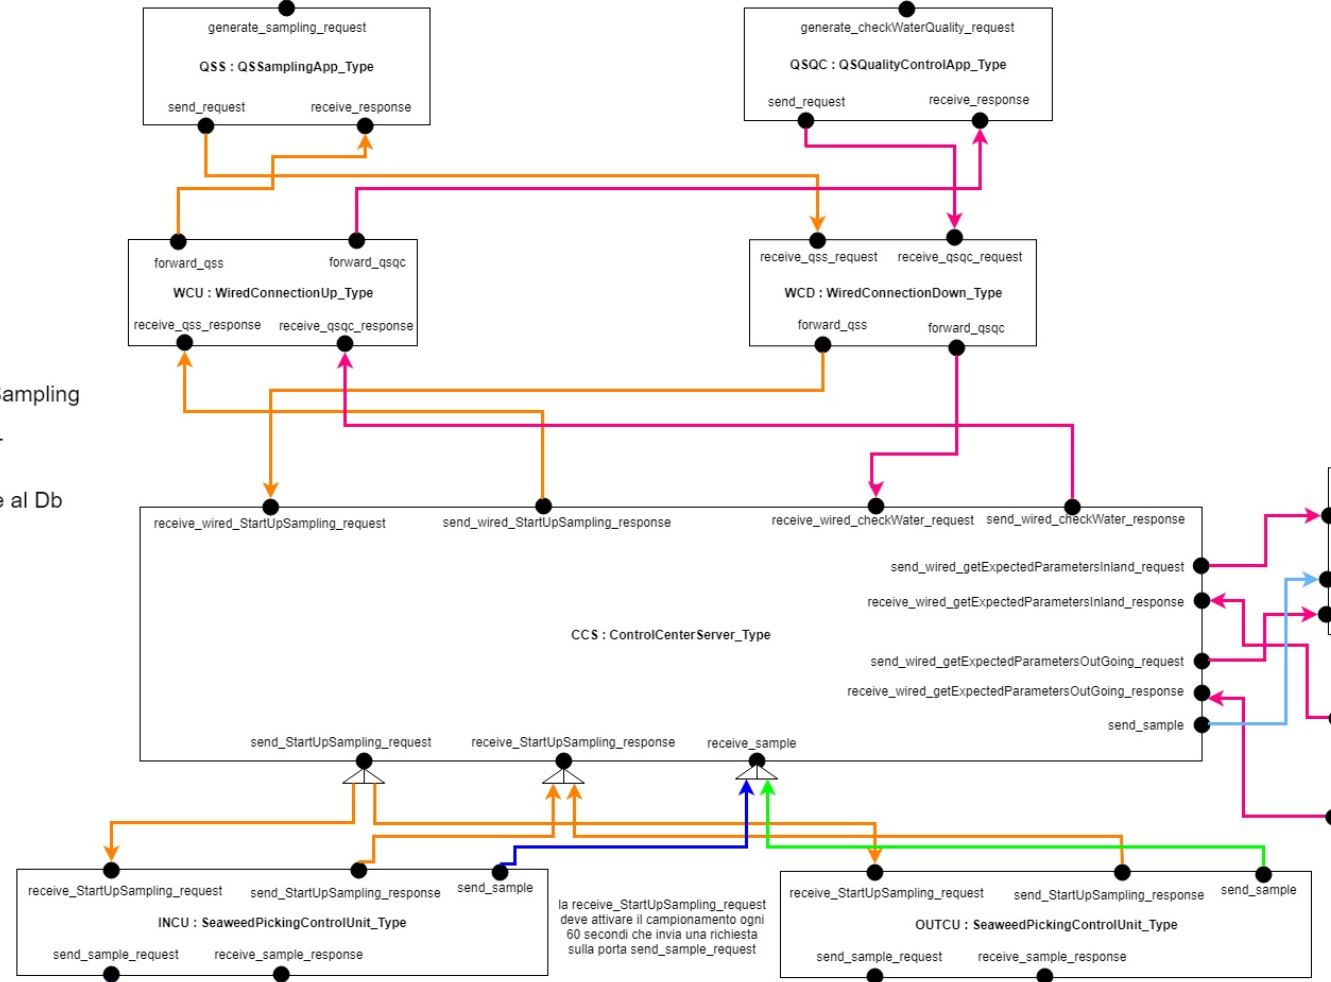
\includegraphics[width=\textwidth]{schermata1.JPG}}
\end{center}
\bigskip
\captionof{figure}{Flow Graph Extract}

\section{Aemilia State Diagram}

In describing the behavior, we created our Diagrams for each Node of the Flow Graph.

\begin{minipage}{0.3\textwidth}
\bigskip
  \makebox[\textwidth]{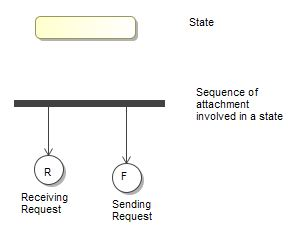
\includegraphics[width= 8cm]				{Legenda.JPG}}
\captionof{figure}{Legenda}
\end{minipage}
\hfill
\begin{minipage}{0.4\textwidth}\raggedleft
We have a block representing the state, a fork under which there is a
sequence of attachments involved within the same state, two circumferences representing these attachments
\end{minipage}
\bigskip

Below you can see an extract of it:

\begin{center}
  \makebox[\textwidth]{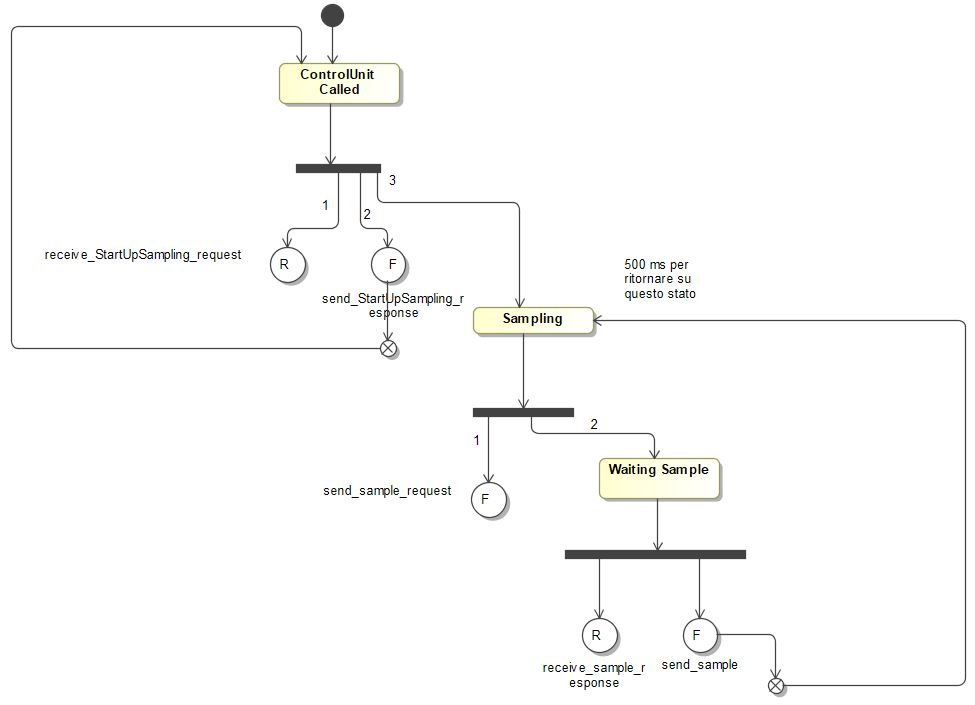
\includegraphics[width=\textwidth]				{stateDiagram.JPG}}
\end{center}
\bigskip
\captionof{figure}{State Diagram Extract}
\bigskip

In this image we see the behavior of the component "SeaweedPicking Control Unit." 

\section{Implementation Of The Model}

Once the behavior of the various nodes, the architecture has been written following the syntax of Aemilia. Below, we will be proposed snippets, coming from previous pictures. 

\lstset {language = C}
\bigskip
\begin{lstlisting}
ELEM_TYPE SeaweedPickingControlUnit_Type(const rate SPCU_send_StartUpSampling_response_rate, const rate SPCU_send_sample_request_rate, 
	const rate SPCU_send_sample_rate, const rate SPCU_delay_rate, const integer sensors_num)

BEHAVIOR

	ControlUnitCalled(void;void) = 
		<receive_StartUpSampling_request, _> . <send_StartUpSampling_response, exp(SPCU_send_StartUpSampling_response_rate)> . Sampling();

	Sampling(void;void) = 
		<send_sample_request, exp(SPCU_send_sample_request_rate)> . WaitingSample();

	WaitingSample(void;void) = 
		<receive_sample_response, _> . <send_sample, exp(SPCU_send_sample_rate)> . Delay();

	Delay(void;void) =
		<delay, exp(SPCU_delay_rate * sensors_num)> . Sampling()


INPUT_INTERACTIONS

	UNI receive_StartUpSampling_request;
		receive_sample_response

OUTPUT_INTERACTIONS 

	UNI send_StartUpSampling_response;
		send_sample;
		send_sample_request
\end{lstlisting}

\section{Test And Analysis Of Results}

After building the model, it was written a file describing the
performance measures to be analyzed. 

\lstset {language = C}
\bigskip
\begin{lstlisting}
MEASURE SeaweedPickingINControlUnitUtilization IS
	ENABLED(INCU.send_StartUpSampling_response) -> TRANS_REWARD(1)
	ENABLED(INCU.send_sample) -> TRANS_REWARD(1)
	ENABLED(INCU.send_sample_request) -> TRANS_REWARD(1);
\end{lstlisting}

After simulating the Model the results are this:

\lstset {language = C}
\bigskip
\begin{lstlisting}
- Value of measure "ControlCenterServerUtilization":
	0.003647

- Value of measure "WaterCompanyServerUtilization":
	0.00271904

- Value of measure "WaterCompanyDiskUtilization":
	0.00225506

- Value of measure "SeaweedPickingINControlUnitUtilization":
	0.0017911

- Value of measure "SeaweedPickingOUTControlUnitUtilization":
	0.0017911

- Value of measure "PurificationSystemServerUtilization":
	0.000463978
\end{lstlisting}

As can be seen from the results the values obtaines from the Aemilia
simulation are very close to those of JMT and the non functional requirements specified at the beginning are all respected.